\section{Project Description}

\subsection{Our Approach}
Our approach to build a modular set of tools that can be used to convert markdown documents into html and pdf format. These tools will be used to develop a command line interface for markdown parsing.

Our approach has two advantages over other solutions:
\begin{itemize}
	\item Developing our software in c++ will result in a product that is faster than solutions
	\item We will develop an API and release the full source code for the components of our product, allowing other programmers to develop their own tools using our code
\end{itemize}
For example, gimli, made by Fredrik Wallgren is written using Ruby~\cite{gimli}, and md-to-pdf made by Simon Hänisch is written in Javascript~\cite{md-to-pdf}. Gimli and md-to-pdf are both command line tools, but we believe that we can speed them up by using c++.

\subsection{Interactions}

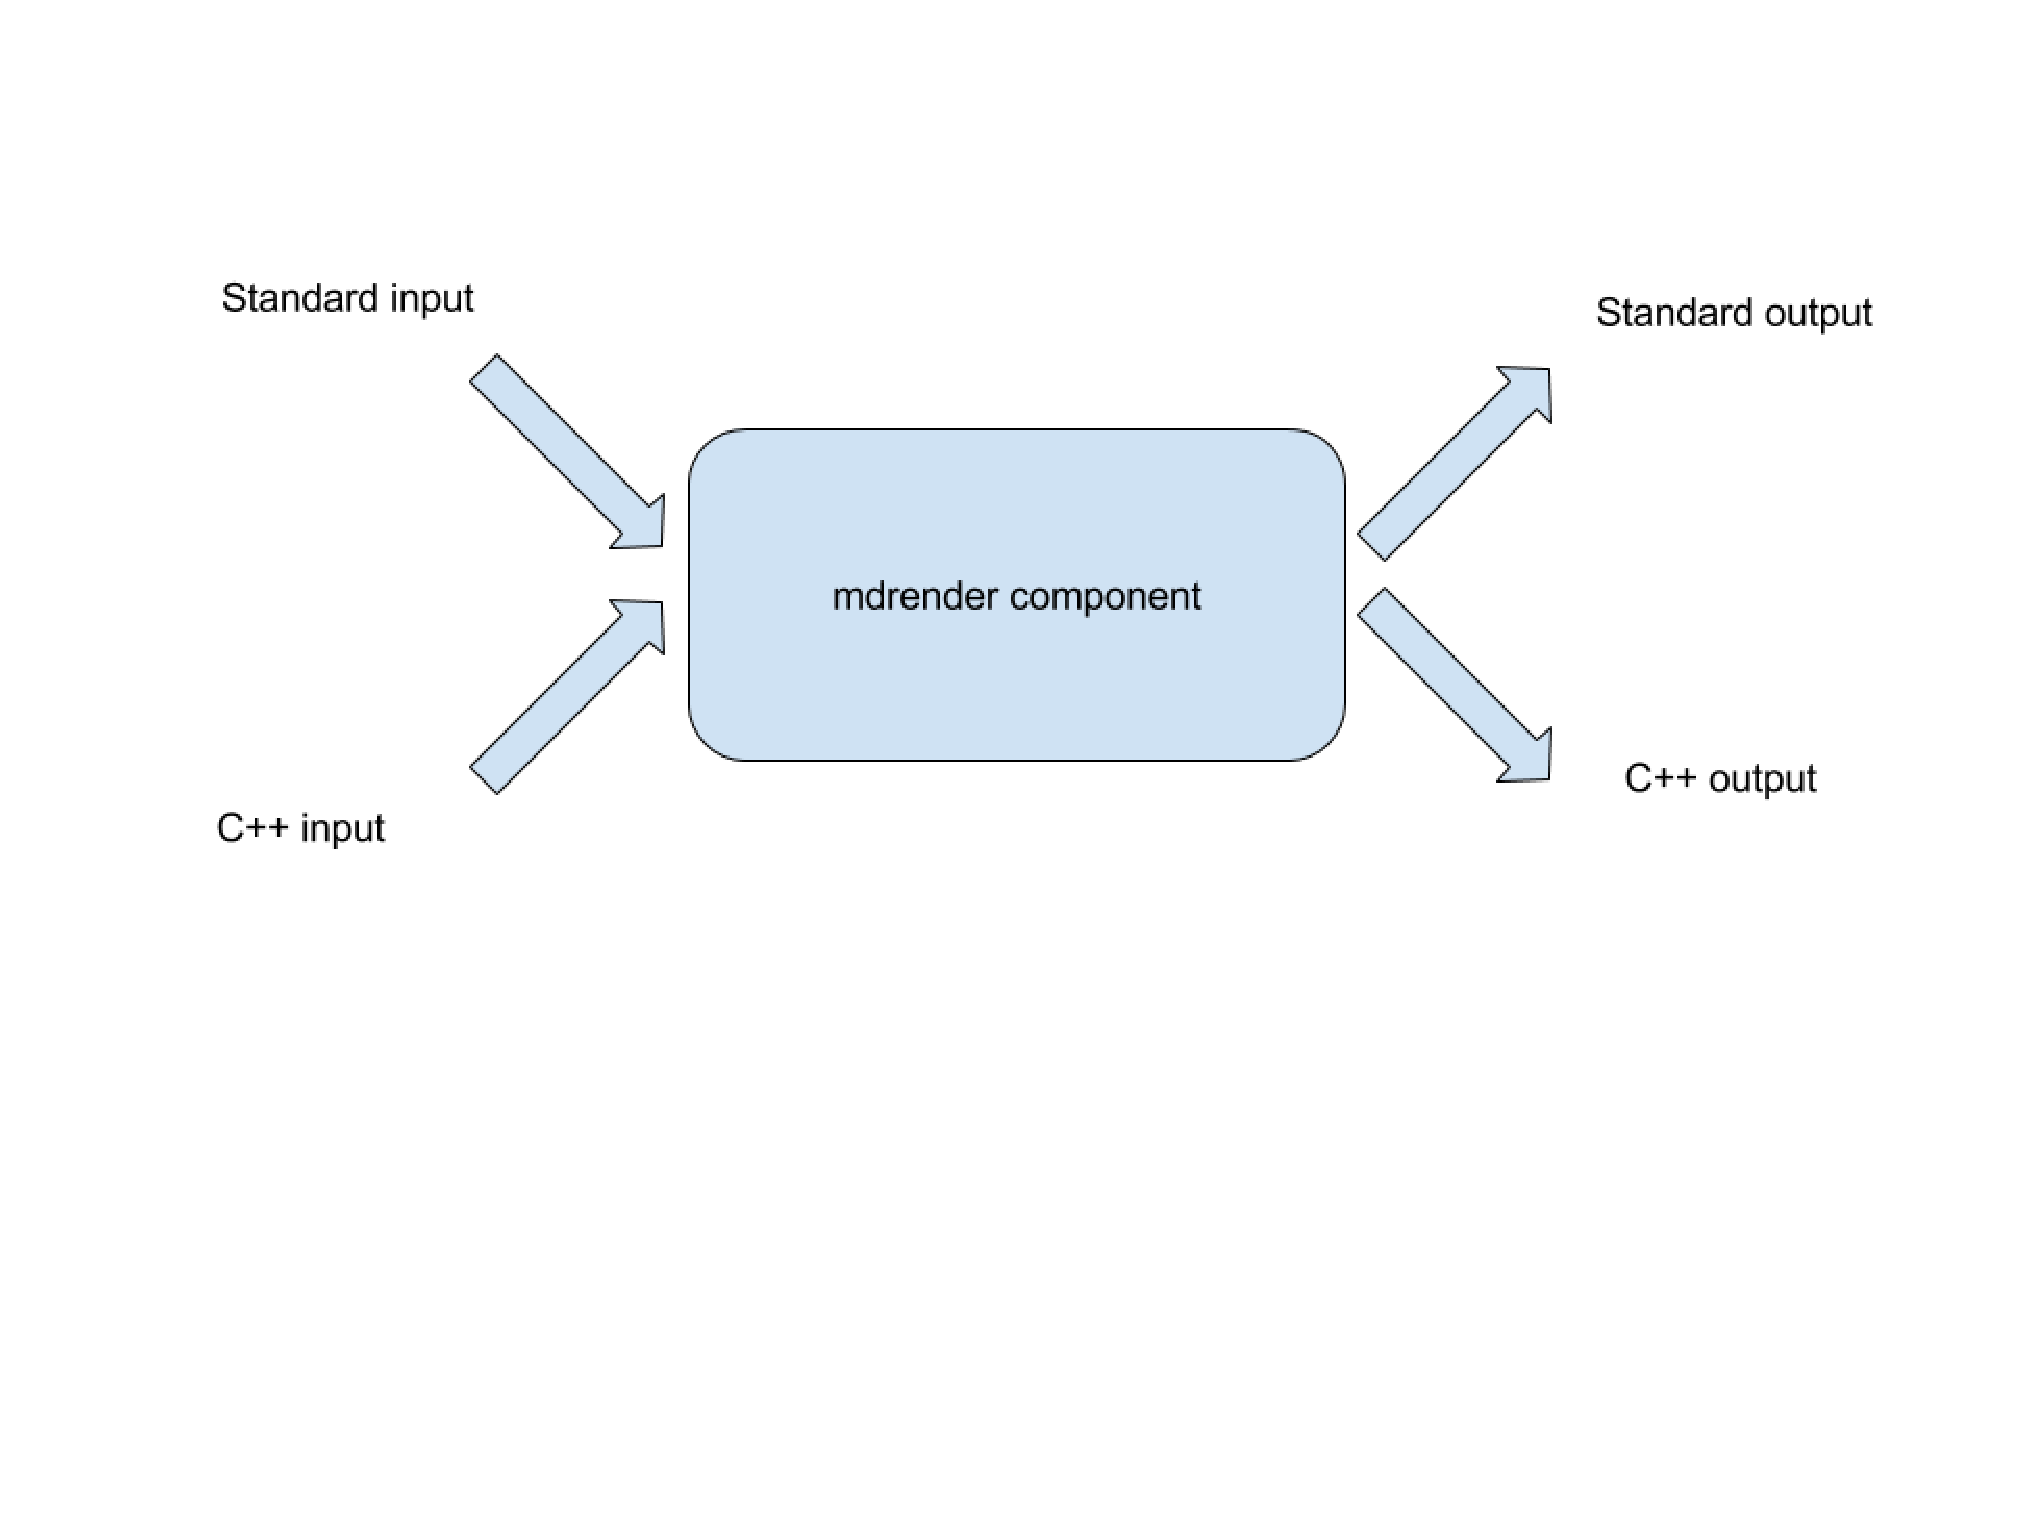
\includegraphics[width=500pt]{images/mdrender_interactions.eps}

This diagram shows how mdrender is designed to be as compatible as possible with other programs by accepting input both via standard in and from other c++ programs as well as outputting data both to standard out and to other c++ programs.

\subsection{Tools}
For this program will be use the following tools and programming languages:
\begin{itemize}
	\item c++ with the g++ compiler
	\item the googletest framework for c++ testing
	\item git and github for source control
\end{itemize}

\subsection{Requirements}

\subsubsection{Functional Requirements}

\begin{itemize}
	\item The system shall be divided into modules that:
		\begin{itemize}
			\item Parse markdown into c++ data
			\item Convert markdown data to pdf data
			\item Convert markdown data to html data
			\item Write pdf and html data to a local file
		\end{itemize}
	\item Each module will be capable of communicating via standard in/out and with other c++ programs
	\item The system will include a command line program that uses all of the modules to convert markdown to pdf or html
\end{itemize}

\subsubsection{Non-functional Requirements}
\begin{itemize}
	\item The system will be optimized to work as quicky as possible
	\item The system will provide a well-documented api to allow others to use the system's functionality
\end{itemize}
